\begin{center}
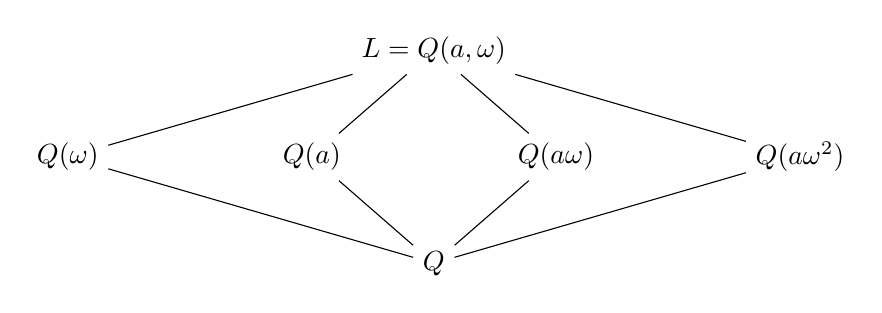
\begin{tikzpicture}[x=1cm,y=1cm]
\node (L) at (4.65,2.7) {$L=\mathbb Q(a,\omega)$};
\node (E0) at (0,1.35) {$\mathbb Q(\omega)$};
\node (E1) at (3.1,1.35) {$\mathbb Q(a)$};
\node (E2) at (6.2,1.35) {$\mathbb Q(a\omega)$};
\node (E3) at (9.3,1.35) {$\mathbb Q(a\omega^2)$};
\node (Q) at (4.65,0) {$\mathbb Q$};
\foreach \j in {0,1,2,3}{\draw (L)--(E\j)--(Q);}
\end{tikzpicture}

\medskip
\begin{tikzpicture}[x=1cm,y=1cm]
\node (one) at (4.65,2.7) {$\{\id\}$};
\node (H0) at (0,1.35) {$\ang{\sigma}=A_3$};
\node (H1) at (3.1,1.35) {$\ang{\tau}$};
\node (H2) at (6.2,1.35) {$\ang{\tau\sigma}$};
\node (H3) at (9.3,1.35) {$\ang{\tau\sigma^2}$};
\node (G) at (4.65,0) {$\ang{\sigma,\tau}=S_3$};
\foreach \j in {0,1,2,3}{\draw (one)--(H\j)--(G);}
\end{tikzpicture}
\end{center}
